

\tikzset{every picture/.style={line width=0.75pt}} %set default line width to 0.75pt        

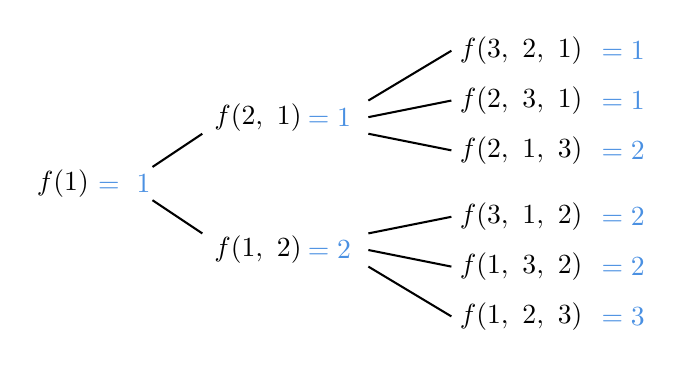
\begin{tikzpicture}[x=0.75pt,y=0.75pt,yscale=-0.8,xscale=0.8]
%uncomment if require: \path (0,300); %set diagram left start at 0, and has height of 300


%Straight Lines [id:da3990866891746605] 
\draw    (200,140) -- (230,120) ;
%Straight Lines [id:da7036777826751123] 
\draw    (200,160) -- (230,180) ;
%Straight Lines [id:da5285761387708318] 
\draw    (330,100) -- (380,70) ;
%Straight Lines [id:da24062270560899968] 
\draw    (330,110) -- (380,100) ;
%Straight Lines [id:da7069018516634579] 
\draw    (330,120) -- (380,130) ;
%Straight Lines [id:da670700481276019] 
\draw    (330,200) -- (380,230) ;
%Straight Lines [id:da9269869048924118] 
\draw    (330,190) -- (380,200) ;
%Straight Lines [id:da6683114952920607] 
\draw    (330,180) -- (380,170) ;

% Text Node
\draw (146,150) node    {$f( 1)$};
% Text Node
\draw (263.5,110) node    {$f( 2,\ 1)$};
% Text Node
\draw (263.5,190) node    {$f( 1,\ 2)$};
% Text Node
\draw (422,70) node    {$f( 3,\ 2,\ 1)$};
% Text Node
\draw (422,100) node    {$f( 2,\ 3,\ 1)$};
% Text Node
\draw (422,130) node    {$f( 2,\ 1,\ 3)$};
% Text Node
\draw (422,170) node    {$f( 3,\ 1,\ 2)$};
% Text Node
\draw (422,200) node    {$f( 1,\ 3,\ 2)$};
% Text Node
\draw (422,230) node    {$f( 1,\ 2,\ 3)$};
% Text Node
\draw (183,150) node  [color={rgb, 255:red, 74; green, 144; blue, 226 }  ,opacity=1 ]  {$=\ 1$};
% Text Node
\draw (306.5,110) node  [color={rgb, 255:red, 74; green, 144; blue, 226 }  ,opacity=1 ]  {$=1$};
% Text Node
\draw (306.5,190) node  [color={rgb, 255:red, 74; green, 144; blue, 226 }  ,opacity=1 ]  {$=2$};
% Text Node
\draw (483.5,70) node  [color={rgb, 255:red, 74; green, 144; blue, 226 }  ,opacity=1 ]  {$=1$};
% Text Node
\draw (483.5,100) node  [color={rgb, 255:red, 74; green, 144; blue, 226 }  ,opacity=1 ]  {$=1$};
% Text Node
\draw (483.5,130) node  [color={rgb, 255:red, 74; green, 144; blue, 226 }  ,opacity=1 ]  {$=2$};
% Text Node
\draw (483.5,170) node  [color={rgb, 255:red, 74; green, 144; blue, 226 }  ,opacity=1 ]  {$=2$};
% Text Node
\draw (483.5,200) node  [color={rgb, 255:red, 74; green, 144; blue, 226 }  ,opacity=1 ]  {$=2$};
% Text Node
\draw (483.5,230) node  [color={rgb, 255:red, 74; green, 144; blue, 226 }  ,opacity=1 ]  {$=3$};


\end{tikzpicture}
